\documentclass[12pt]{article}
\usepackage{amsmath, amssymb}
\usepackage{amsthm}
\usepackage{hyperref}
\usepackage{MnSymbol}
%%\usepackage[pdftex]{graphicx}
\usepackage{enumerate}
\usepackage{amsmath}
\usepackage{amssymb}
\usepackage{multicol}
\usepackage{algpseudocode}
\usepackage{algorithm}


\usepackage[final]{graphicx}
\usepackage{subcaption}
\renewcommand{\phi}{\varphi}
\newcommand{\rarrow}{\rightarrow}
\usepackage{ listings}
\title{COMP 576 Deep Learning}

\author{Guangyuan Yu(gy12)}


\begin{document}
\maketitle

\section{Visualizing A cnn}

\subsection{a}
\subsection{b}
After 17400 steps, Train accuracy: 0.96875
test accuracy: 0.57
After 17500 steps, Train accuracy: 0.921875
test accuracy: 0.561
After 17600 steps, Train accuracy: 0.9375
test accuracy: 0.569
After 17700 steps, Train accuracy: 0.921875
test accuracy: 0.554
After 17800 steps, Train accuracy: 0.9375
test accuracy: 0.564
After 17900 steps, Train accuracy: 0.9375
test accuracy: 0.564
test accuracy 0.555
\begin{figure}[H]
  \caption{center}
  \centering
    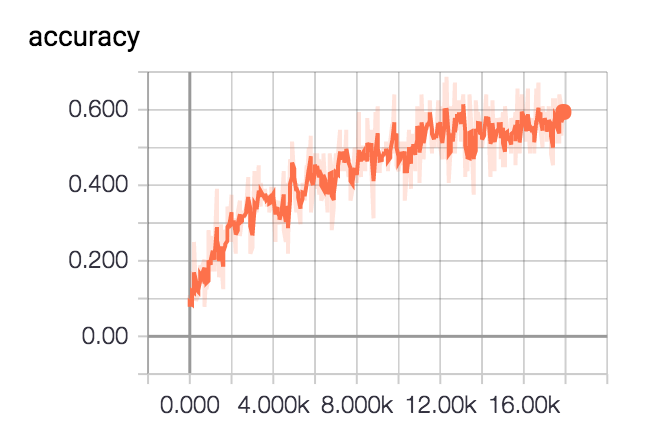
\includegraphics[scale=1]{train.png}
\end{figure}
\begin{figure}[H]
  \caption{center}
  \centering
    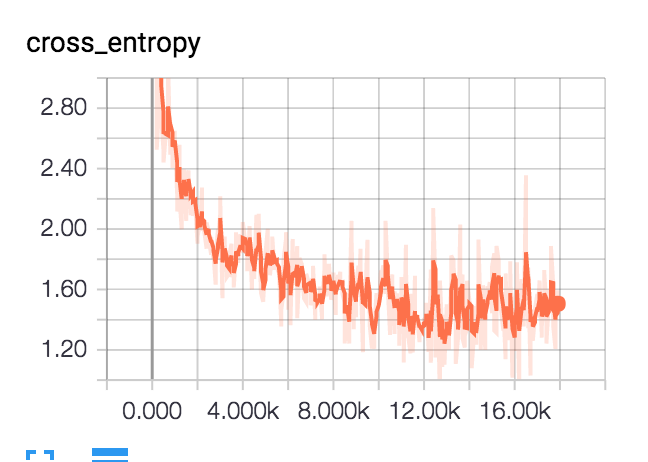
\includegraphics[scale=1]{cross.png}
\end{figure}
\begin{figure}[H]
  \caption{center}
  \centering
    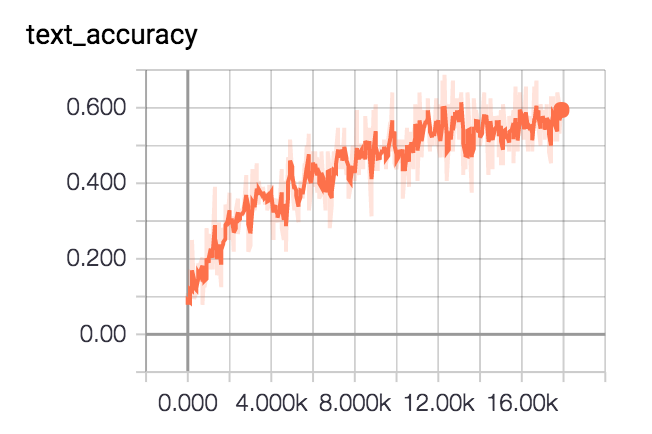
\includegraphics[scale=1]{test.png}
\end{figure}

\subsection{c visuzlization}
The weight is shown here:
\begin{figure}[H]
  \caption{center}
  \centering
    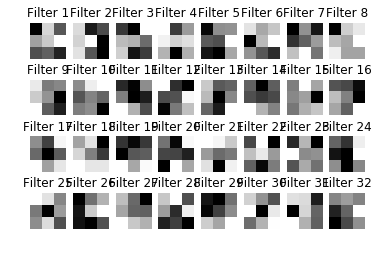
\includegraphics[scale=1]{123.png}
\end{figure}


The activation is shown here: I use a test picture as input and see what it looks like after the first layer, I showed 32 filters here.
\begin{figure}[H]
  \caption{center}
  \centering
    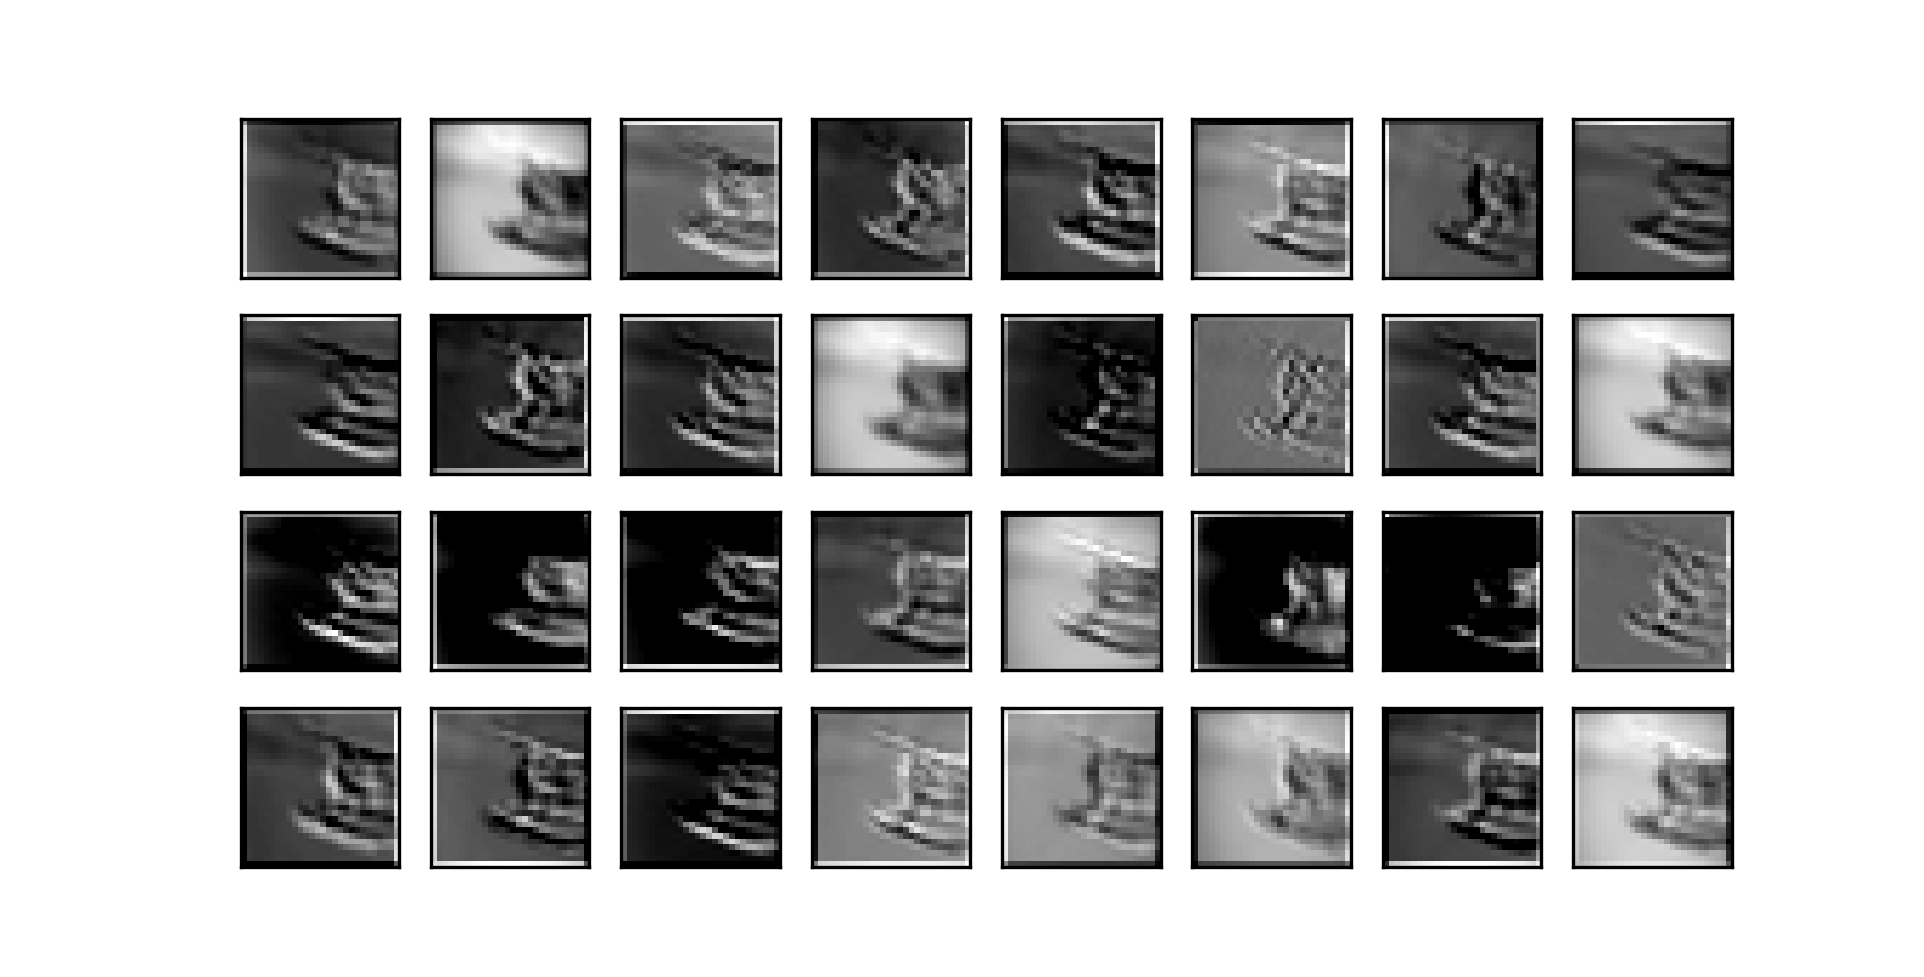
\includegraphics[scale=1]{Figure1.png}
\end{figure}
The activation is shown here: I use a test picture as input and see what it looks like after the second layer, I showed 64 filters here.
\begin{figure}[H]
  \caption{center}
  \centering
    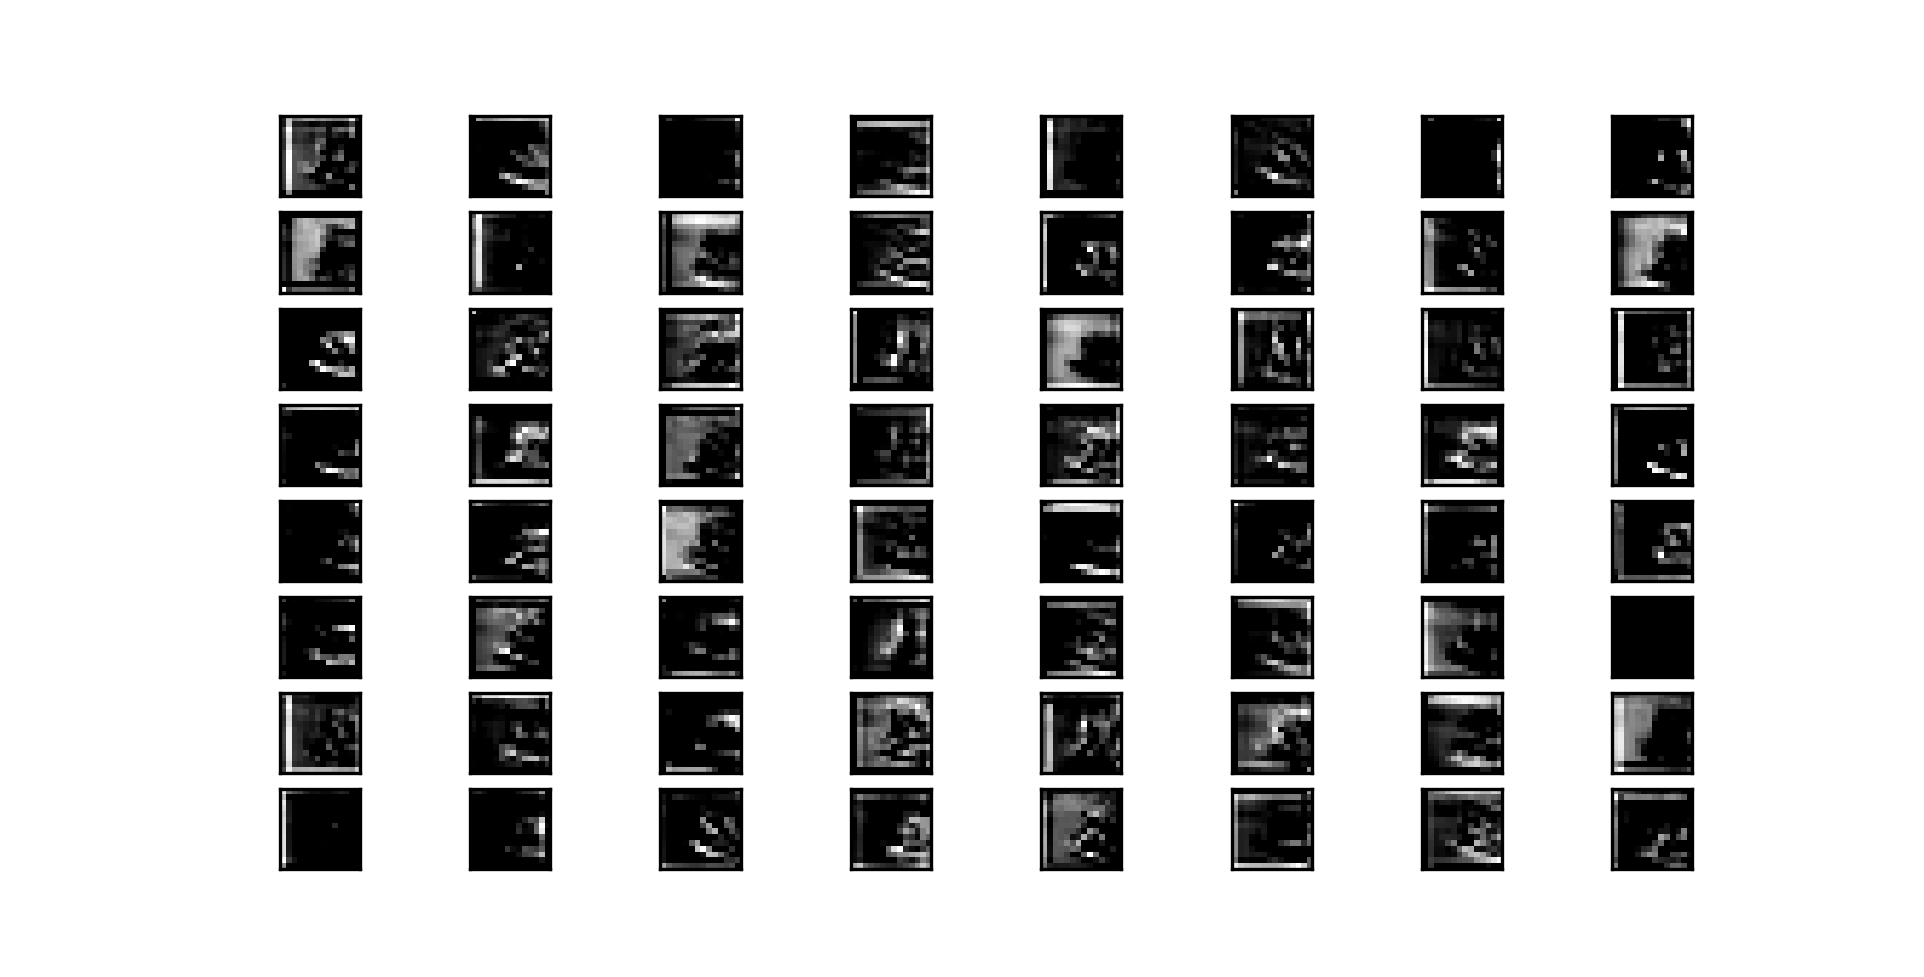
\includegraphics[scale=1]{Figure2.png}
\end{figure}



\section{2 paper}
key ideas:
convolutional neural network has very good performance in the field of number recognition and face detection. CNN has good performance has good performance in classification problems have been shown in many papers. The re-popular of CNN depends on several reasons: 1 the millions training sets with labels, 2 GPU acceleration, 3 optimizing strategy? like dropout method.
But people has few understanding about how the CNN works. It i like a black box, the fine-tune of parameter highly depends on luck, which is not an attitude of science.
In this paper, the author use a deconvoluational network to visualize the CNN and see how the features change with layer and did some test about the sensitivity. 
deconvoluational network has three part: unpooling, rectification, filtering. The pooling is not reversible? so the CNN will remember the max pool position and use the position for unpooling, other places are filled with 0.

The training result shows that the higher layer has higher nonlinearity?the feathers in the same layer have similar result, all the features are the characteristic of the original picture. 
For parallel translation? the CNN has good invariance? but for rotation, the performance is bad. 
The author also did test on sensitivity which will use a box the hide parts of the picture. When the face of the dog is hidden, the picture will be labeled as tennis, but when other parts are labeled, the picture are still recognized as dog. 
\subsection{optional}
I rotate, flip  the testset and compare the result with the original result to see the tolerance of the system.
The python file to rotate and flip is called rotate.py.
\begin{lstlisting}
The original result is 
After 17400 steps, Train accuracy: 0.953125
test accuracy: 0.56
After 17500 steps, Train accuracy: 0.890625
test accuracy: 0.552
After 17600 steps, Train accuracy: 0.90625
test accuracy: 0.57
After 17700 steps, Train accuracy: 0.953125
test accuracy: 0.567
After 17800 steps, Train accuracy: 0.984375
test accuracy: 0.572
After 17900 steps, Train accuracy: 0.90625
test accuracy: 0.568
test accuracy 0.567
\end{lstlisting}

After I flip the testset unside down, we can see the result didn't change too much. 
\begin{lstlisting}
After 17300 steps, Train accuracy: 1
test accuracy: 0.582
After 17400 steps, Train accuracy: 1
test accuracy: 0.593
After 17500 steps, Train accuracy: 0.921875
test accuracy: 0.586
After 17600 steps, Train accuracy: 0.984375
test accuracy: 0.582
After 17700 steps, Train accuracy: 0.953125
test accuracy: 0.582
After 17800 steps, Train accuracy: 0.96875
test accuracy: 0.589
After 17900 steps, Train accuracy: 0.96875
test accuracy: 0.584
test accuracy 0.585
\end{lstlisting}



After I flip the testset with left and right, we can see the result didn't change too much. 
\begin{lstlisting}
zuooyu 7400 steps, Train accuracy: 0.953125
test accuracy: 0.578
After 17500 steps, Train accuracy: 0.96875
test accuracy: 0.58
After 17600 steps, Train accuracy: 0.984375
test accuracy: 0.585
After 17700 steps, Train accuracy: 0.96875
test accuracy: 0.585
After 17800 steps, Train accuracy: 0.984375
test accuracy: 0.588
After 17900 steps, Train accuracy: 0.984375
test accuracy: 0.584
test accuracy 0.578
\end{lstlisting}

After I rotate the picture of 90 degree, we can see the accuracy drop a lot, which is the same in the paper that the CNN has low invariance in rotation. 
\begin{lstlisting}

After 17400 steps, Train accuracy: 0.953125
test accuracy: 0.188
After 17500 steps, Train accuracy: 0.9375
test accuracy: 0.177
After 17600 steps, Train accuracy: 0.953125
test accuracy: 0.174
After 17700 steps, Train accuracy: 0.953125
test accuracy: 0.178
After 17800 steps, Train accuracy: 0.953125
test accuracy: 0.184
After 17900 steps, Train accuracy: 0.9375
test accuracy: 0.178
test accuracy 0.174
\end{lstlisting}








\section{3RNN}
\subsection{a}

\subsection{b}

plot of train/test accuracy and the loss
\begin{figure}[H]
  \caption{center}
  \centering
    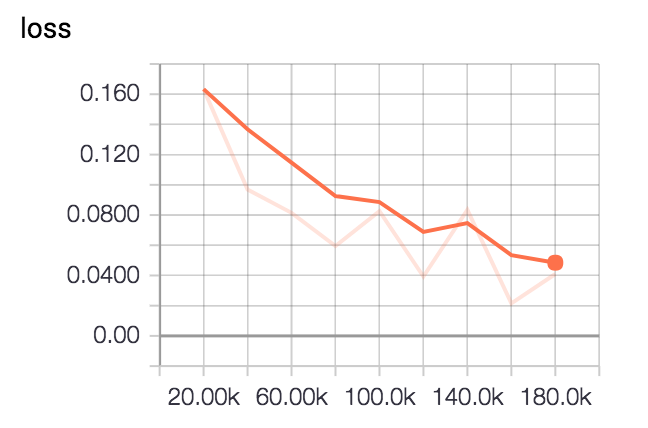
\includegraphics[scale=1]{3los.png}
\end{figure}

\begin{figure}[H]
  \caption{center}
  \centering
    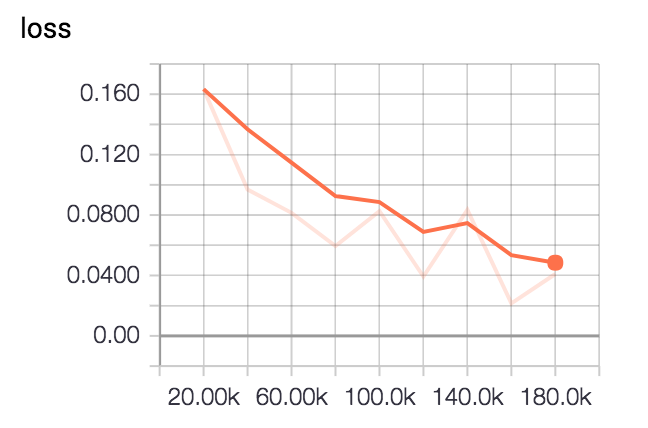
\includegraphics[scale=1]{3test.png}
\end{figure}

\begin{figure}[H]
  \caption{center}
  \centering
    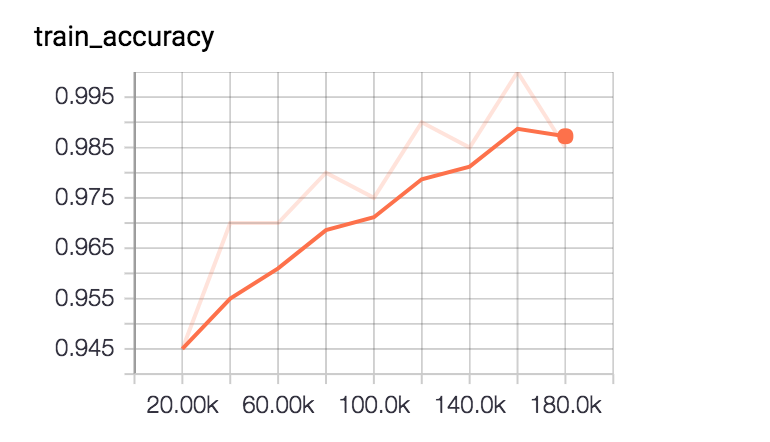
\includegraphics[scale=1]{3train.png}
\end{figure}









With 100 hidden unit, here is the training result.

\begin{lstlisting}

lstmCell = rnn.BasicLSTMCell
Iter 1904000, Minibatch Loss= 0.04613, Training Accuracy= 0.98571, 
Test Accuracy= 0.97530
Iter 1932000, Minibatch Loss= 0.03805, Training Accuracy= 0.98929, 
Test Accuracy= 0.97770
Iter 1960000, Minibatch Loss= 0.03214, Training Accuracy= 0.99286, 
Test Accuracy= 0.97670
Iter 1988000, Minibatch Loss= 0.04148, Training Accuracy= 0.98214, 
Test Accuracy= 0.97700
Optimization finished
Testing Accuracy: 0.9736
lstmCell = rnn.BasicRNNCell(nHidden)
Iter 1904000, Minibatch Loss= 0.01676, Training Accuracy= 0.99643, 
Test Accuracy= 0.97290
Iter 1932000, Minibatch Loss= 0.03559, Training Accuracy= 0.99286, 
Test Accuracy= 0.97730
Iter 1960000, Minibatch Loss= 0.01943, Training Accuracy= 0.99643, 
Test Accuracy= 0.97540
Iter 1988000, Minibatch Loss= 0.01475, Training Accuracy= 1.00000, 
Test Accuracy= 0.97530
Optimization finished
Testing Accuracy: 0.9773

lstmCell = rnn.GRUCell(nHidden)
Iter 1904000, Minibatch Loss= 0.06418, Training Accuracy= 0.98214, 
Test Accuracy= 0.97820
Iter 1932000, Minibatch Loss= 0.03376, Training Accuracy= 0.99286, 
Test Accuracy= 0.97550
Iter 1960000, Minibatch Loss= 0.08083, Training Accuracy= 0.96786, 
Test Accuracy= 0.96350
Iter 1988000, Minibatch Loss= 0.03238, Training Accuracy= 0.98571, 
Test Accuracy= 0.97660
Optimization finished
Testing Accuracy: 0.9728
\end{lstlisting}
We can see that the test accuracy of LSTM and GRU and BasicRNN almost the same, but BasicRNN has slightly overfitting. 



when we change the hidden unit and compare the result, we find the 500 hidden unit is better than 100 unit.

\begin{lstlisting}
Iter 2920000, Minibatch Loss= 0.02911, Training Accuracy= 0.99000, 
Test Accuracy= 0.97930
Iter 2940000, Minibatch Loss= 0.05172, Training Accuracy= 0.98500, 
Test Accuracy= 0.97960
Iter 2960000, Minibatch Loss= 0.02052, Training Accuracy= 0.99500, 
Test Accuracy= 0.97960
Iter 2980000, Minibatch Loss= 0.04976, Training Accuracy= 0.98500, 
Test Accuracy= 0.97750
Optimization finished
Testing Accuracy: 0.9792



Iter 2920000, Minibatch Loss= 0.02698, Training Accuracy= 0.99500,
 Test Accuracy= 0.97870
Iter 2940000, Minibatch Loss= 0.02429, Training Accuracy= 0.99000, 
Test Accuracy= 0.97870
Iter 2960000, Minibatch Loss= 0.02284, Training Accuracy= 0.99500, 
Test Accuracy= 0.98030
Iter 2980000, Minibatch Loss= 0.00857, Training Accuracy= 1.00000,
 Test Accuracy= 0.98110
Optimization finished
Testing Accuracy: 0.9809
\end{lstlisting}









\subsection{compare with CNN in HW1}
In HW1, we also use this dataset. in that part, I use tanh function and use about 106 secod to train 5500 steps and get an test accuracy of 0.945, here with 200 hidden unit and the same learning rate and same optimizer, RNN get slightly higher accuracy of 0.986 when trained 6000 times. If we trained it 1500 times, the accuracy is about 0.98. So I think RNN is better than CNN. The time consumption is almost the same.








\begin{lstlisting}

\end{lstlisting}



			\end{document}

